\section{Method Overview}
\label{sec:Method_Overview}

\noindent Figure~\ref{fig:method_and_prototype_schematic} illustrates a high-level, domain-agnostic schematic of our method and prototype. Domain experts, who are the method's primary stakeholders, use OWL to define domain concepts and their relationships; SWRL and Prolog to define rules; and PRISM's modeling and property specification languages to define, respectively, DTMC and PCTL templates. Model builders, who are also primary stakeholders, use a high-level DSL to encode system specifications for model checking. We note that domain knowledge is formalized once and subsequently reused to support the verification of multiple system specifications.

\begin{figure*}
\centering
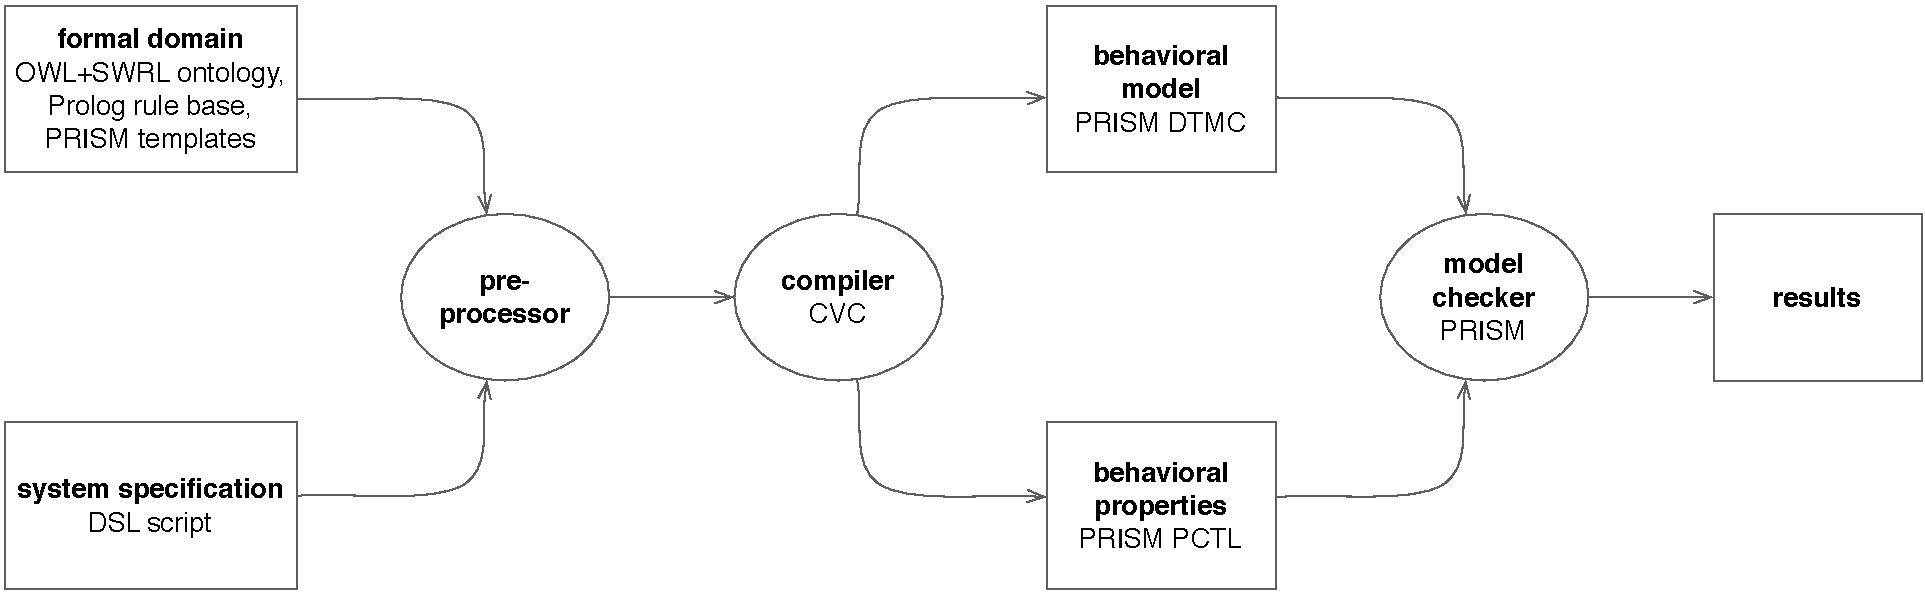
\includegraphics[scale=0.54]{img/schematic.pdf}
\caption{A high-level, domain-agnostic schematic of our method and prototype. Rectangular and oval shapes represent data and processes, respectively; and bold and normal text distinguishes method from prototype, respectively.}
\label{fig:method_and_prototype_schematic}
\end{figure*}

\subsection{An Example Mission}
\label{sec:An_Example_Mission}

\noindent With our prototype, model builders use a domain-specific YAML dialect to encode mission plans comprising UAV \emph{assets} and the \emph{action workflows} assigned to those assets. The YAML code in Listing~\ref{lst:Mission_A} specifies Mission~A, an example mission that is representative of the~58 mission plans developed for this project.

\begin{lstlisting}[caption={YAML code for Mission~A},label=lst:Mission_A]
Action:
  TraversePathSegmentAction:
    - id: TPSA1
      duration: 60
      coordinates: [-118.27017, 34.04572,
        -118.27279, 34.04284]
    - id: TPSA2
      duration: 60
      coordinates: [-118.2739, 34.03928]
      preconditions: [TPSA1, TPSA3]
    - id: TPSA3
      duration: 60
      coordinates: [-118.26482, 34.03332,
        -118.27383, 34.03824]
    - id: TPSA4
      duration: 60
      coordinates: [-118.28204, 34.0376]
      preconditions: [TPSA3]
  PhotoSurveillanceAction:
    - id: PSA5
      duration: 50
      preconditions: [TPSA3]
Asset:
  Hummingbird:
    - id: H1
      actions: [TPSA1, TPSA2]
    - id: H2
      actions: [TPSA3, TPSA4, PSA5]
\end{lstlisting}

Mission~A comprises two \emph{Hummingbird} assets (lines~24--28 in Listing~\ref{lst:Mission_A}); a single \emph{photo surveillance action} (lines~19--22), which is a type of \emph{sensor action}; and four \emph{path segment traversal actions} (lines~2--18), which are \emph{kinetic actions}. A path segment traversal action instructs the executing UAV to traverse a path between two waypoints. For each such action, the latitudes and longitudes of the delineating waypoints are stored in an array and indexed in succession; in other words, the latitude of waypoint one is followed by the longitude of waypoint one, which is in turn followed by the latitude of waypoint two, etc. We note that the end coordinates of an action~\emph{a} constitute the start coordinates of an action~\emph{b} if~\emph{a} precedes~\emph{b}, and both~\emph{a} and~\emph{b} are assigned to the same asset; for example, the end coordinates of action \texttt{TPSA1} (line~6) constitute the implied start coordinates of action \texttt{TPSA2}, which succeeds \texttt{TPSA1} in the sequence of kinetic actions assigned to asset \texttt{H1} (line~26).

The mission concepts described above will be elaborated as we proceed to analyze our method and prototype.

\subsection{From Specification to Verification}

\noindent For any given mission specification, a \emph{cascading verification compiler} (CVC) synthesizes both the DTMC and PCTL artifacts corresponding to that specification. Artifacts are synthesized as follows:

\begin{enumerate}

\item Mission specifications encoded in YAML are transformed by the CVC into ABox assertions. During this preprocessing phase, the CVC uses geographic coordinates from mission specifications, and data (pertaining to operational environments) from external sources, to perform geodetic calculations.\footnote{Geodetics is a branch of applied mathematics that deals with the size and shape of the Earth.} The equations that support these calculations are hard-coded in the CVC; for example, the compiler comprises geodesic equations that establish the occurrence, and calculate the duration, of threat area incursions committed by UAVs. Geographic information resulting from preprocessing is integrated with the generated ABox.

\item We use Pellet, a sound and complete semantic reasoner~\cite{Sirin_2007}, to verify the generated ABox against the TBox defined by domain experts. In doing so, the reasoner ensures that mission constructs encoded in YAML are consistent with OWL+SWRL axioms. Inconsistencies between TBox and ABox signify an invalid mission specification, which causes the compilation process to terminate with an error. If consistency is deduced, then the reasoner proceeds to generate inferences from explicitly encoded domain knowledge; for example, if geodetic calculations establish the occurrence of a threat area incursion, then the asset committing that incursion is inferred to be a \emph{threatened asset}.

\item Inferred ontological knowledge is transformed by the CVC into Prolog facts. The compiler for SWI-Prolog---an open source implementation of Prolog~\cite{SWI_Prolog}---inputs the generated fact-base, and the Prolog rule-base defined by domain experts, and proceeds to generate inferences; for example, the last kinetic action in an action workflow is inferred to be a \emph{default terminal action}. The CVC uses Prolog inferences, in conjunction with explicit and inferred ontological knowledge, to synthesize DTMC and PCTL artifacts from predefined templates.

\end{enumerate}

PRISM inputs the synthesized artifacts, verifies the system model against its desired behavioral properties, and returns logical and probabilistic results from the verification. If the results are deemed acceptable by the model builder(s), then the mission can be scheduled for real-world execution (via some process that is outside the scope of our method).
